% >>>>>>>>>>>>>>>>>>
\slide{}{
\begin{itemize}
    \item Teoria dos Jogos
    \begin{itemize}
        \item Jogos na Forma Normal
        \item Jogos na Forma Extensiva
    \end{itemize}
    \item Aprendizado por Reforço
    \begin{itemize}
        \item Processo de Decisão Markoviano
        \item Q-Learning
    \end{itemize}
\end{itemize}
}


\slide{Jogos na Forma Normal}{
Jogos na Forma Normal podem ser descritos como uma tupla (n, $A_{1,...n}$, $R_{1,...,n}$)
\begin{itemize}
    \item n é uma coleção de participantes, chamados de jogadores
    \item $A_{k}$ é o conjunto finito de ações disponíveis ao jogador;
    \item $R_{k}: A_{1}\times ... \times A_{n}$ $\xrightarrow{} \mathbf{a}$ é a função de recompensa individual para o jogador K, que especifica a recompensa recebida para um jogada $\mathbf{a} \in A_{1}\times ... \times A_{n}$
    \end{itemize}
}
\slide{Jogos na Forma Normal}{

\begin{itemize}
    \item A combinação de escolhas dos jogadores constitui um perfil de ações $\mathbf{a} \in \mathbf{A}$.
    \item Uma estratégia $\sigma_{k}: A_{k}\xrightarrow{}[0,1]$ é o conjunto de distribuições de probabilidades de $A_{k}$;
    \item Uma estratégia é dita pura se $\sigma_{k}(a)=1$ para alguma $\mathbf{a} \in A_{k}$
    \item Um perfil estratégico $\sigma = (\sigma_{1}, ..., \sigma_{k})$ é um vetor contendo uma estrategia para jogador. 
    \item A recompensa esperada para um jogador $k$ em um perfil estratégico $\sigma$ é dada por: 
    \begin{equation}
        R_{k}(\sigma)= \sum_{a\in \mathbb{A}}^{} \prod_{j=1} ^{n} \sigma_{j}(a_{j})R_{k}(\textbf{a})
    \end{equation}
    \end{itemize}
}
\begin{frame}{Jogos na Forma Extensiva}

    \begin{figure}
        \centering
        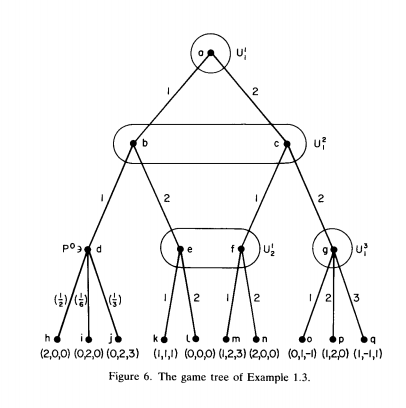
\includegraphics[scale=0.5]{img/Exemplo_Jogos_Extendidos.png}
        \caption{Exemplo de jogo na forma Extensiva}
    \end{figure}
   
\end{frame}


\slide{Equilíbrio em Jogos}{

\begin{enumerate}
    \item A estratégia $\sigma_{k} \in \mu(A_{k})$ é a melhor estratégia se:
        \begin{equation}
            R_{k}(\sigma_{-k} \cup \sigma_{k})\geq R_{k}(\sigma_{-k}\cup \sigma_{k}^{'}) \forall{} \sigma_{k}^{'} \in \mu(A_{k})
        \end{equation}
    \item Definimos o Equilíbrio de Nash como um perfil estratégico $\sigma = (\sigma_{1}, ..., \sigma_{n})$ no qual, para cada jogador k, a estratégia $\sigma_{k}$ é a melhor resposta para aquele jogador. 
\end{enumerate}

}



\slide{Aprendizado por Reforço}{
\begin{itemize}
    \item Aprendizado através da experimentação.
    \item Postergação da recompensa.
    \item Explorar ou Agir conforme o conhecimento adquirido. 
    
\end{itemize}
}



\slide{Processo de Decisão de Markov}{
Um processo de decisão de Markov pode ser descrito como uma tupla $(S, A, T, R, \gamma)$
\begin{itemize}
    \item $S$ é o conjunto de estados do ambiente
    \item $A$ é o conjunto finito de ações do agente
    \item $T$ é a função de transição de estados $f: S\times A\times S \xrightarrow{} [0,1]$
    \item $R$ é a função de recompensa $R: S \times A \times S -> \mathbb{R}$
    \item $\gamma$ é o fator de desconto 
    
\end{itemize}
}

\slide{Processo de Decisão de Markov}{

\begin{itemize}
    \item $S_{t}$ é o sinal de estado que descreve o ambiente no instante t.
    \item O agente pode alterar o estado a cada instante tomando uma ação $a_{k} \in A$.
    \item Agente transita de um estado $s_{t}$ para um estado $s_{t+1} \in S$, de acordo com a função T
    \item A probabilidade que o agente chegue em $S_{t+1}$ ao agir de forma $a_{t}$ é dada por $T(s_{t}, a_{t}, s_{t+1})$ e a recompensa associada é dada por $T(s_{t}, a_{t}, s_{t+1})$
    \item Para cada ação o agente recebe uma recompensa $r_{t} \in \mathbb{R}$ dada por $R(s_{t}, a_{t}, s_{t+1})$
    
\end{itemize}
}


\slide{Processo de Decisão de Markov}{

    O objetivo do agente é maximizar a cada instante t o retorno descontado esperado: 
    \begin{equation}
        R_{t} = E(\sum_{j=0}^{\infty}\gamma^{j}r_{t+j})
    \end{equation}
}

\slide{Processo de Decisão de Markov}{
   \begin{itemize}
       \item Para maximizar $R_{t}$, calula-se \textit{action-value function}(Q-function), 
       \item $Q^{h}: S \times A \xrightarrow{} \mathbb{R}$
   \end{itemize}  
    \begin{equation}
        Q^{h}=  E(\sum_{j=0}^{\infty}\gamma^{j}r_{t+j+1}|s_{t}= s, a_{t}=a, h)
    \end{equation}
}

\slide{Processo de Decisão de Markov}{
   Podemos entender a tarefa de aprendizagem como o calculo da função $Q^{*}$, definida como Q-function ótima: 
    \begin{equation}
    Q^{*}= arg\max_{h}Q^{h}(s,a)
    \end{equation}
   

}
\slide{Processo de Decisão de Markov}{
    \begin{itemize}
        \item A partir de $Q^{*}$, o agente pode adotar uma estratégia determinística e gananciosa, escolhendo para cada estado a ação que retorna o maior valor:
        
        \begin{equation}
            h^{*}=arg \max_{a}Q(s,a)
        \end{equation}
        \item Como aprender $Q^{h}(s,a)$?
    \end{itemize}
    
    
    
}


\slide{Q-Learning}{
    \begin{enumerate}
    \item Observa seu estado atual $x_{n}$
    \item seleciona e performa a ação $a_{n}$
    \item observa o estado subsequente $y_{n}$
    \item recebe uma recompensa imediata $r_{n}$, e 
    \item ajusta o valor $Q_{n-1}$ utilizando um fator de aprendizado $\alpha$ na forma:
    \begin{equation}
        Q_{n}(x,a) = .
        \begin{cases}
            (1-\alpha_{n})Q_{n-1}(x,a)+\alpha_{n}[r_{n}+\gamma Q_{n-1}(y_{n}),\\ $se x= $x_{n} $e a= $a_{n}\\
            Q_{n-1}(x,a),$caso contrario$\\
        \end{cases}
    \end{equation}
    \\no qual:
    \begin{equation}\label{eq:1}
           Q_{n-1}\equiv \max_{b}{Q_{n-1}(y,b)}
    \end{equation}
    \end{enumerate}
}

\slide{Q-Learning}{
    A garantia de optimalidade de Q-learning, ou seja que a função $Q_{n}(x,a)$ converge para $Q^{*}(x,a)$ a medida que $n\xrightarrow{}\infty$ é dada pelo teorema:
    
    Dada recompensas limitadas $|r_n|<\mathbb{R}$, taxas de aprendizado $0\leq\alpha<1$ e:
    \begin{equation}
        \sum_{i=1}^\infty\alpha Q_{n^{i}(x,a)}= \infty, \sum_{i=1}^\infty[\alpha Q_{n^{i}(x,a)}]^{2}<\infty, \forall{x}, \alpha,
    \end{equation}
    
    então $Q_{n}(x,a)\xrightarrow{}Q^{*}(x,a)$ quando $n\xrightarrow{} \infty, \forall{x}, \alpha$, com probabilidade 1.
}

\slide{Q-Learning}{
\begin{itemize}
    \item Equilibrio entre exploração e explotação
    \item Politicas GLIE(\textit{Greedy in the limit with infinite exploration})
    \item $1-\epsilon(s)$, sendo $\epsilon(s)=c/n(s)$ e $0<c<1$.
\end{itemize}
   
  
}


